\documentclass[10pt]{report}

\usepackage{fontspec}
\usepackage[english,frenchb]{babel}
\usepackage{titlesec}
\usepackage{titling}
\usepackage[table,xcdraw]{xcolor}
\usepackage{geometry}
\usepackage{listings}
\usepackage{graphicx}
\usepackage{pgf-umlcd}
\usepackage{blindtext}
\usepackage{tikz}
\usepackage{mathtools}


\setmainfont{Minion Pro}
\newfontfamily\headingfont{Myriad Pro}
\newfontfamily\codefont{Ubuntu Mono}

\titleformat{\chapter}[display]
{\bfseries\headingfont\filleft}
{\scalebox{0.8}[1.2] }
{0pc}
{\titlerule \vspace{0.3pc} \Huge\scalebox{0.8}[1.2]}
\titleformat{\section}[display]
{\bfseries\headingfont\filright}
{}
{0pt}
{\Large\scalebox{0.9}[1.4]}
\titlespacing{\chapter}
{0pc}{0pc}{6pc}[0pc]
\titlespacing{\section}
{0pc}{-1pc}{0pc}[0pc]


\setlength\parindent{0pt}
\setlength\parskip{6pt}

\makeatletter
\newcommand{\globalcolor}[1]{\color{#1}\global\let\default@color\current@color}
\makeatother
\definecolor{TextColor}{rgb}{0.15,0.14,0.13}
\AtBeginDocument{\globalcolor{TextColor}}

\geometry{
 a4paper, 
 voffset=0mm,
 headheight=0mm,
 headsep=0mm,
 left=17mm,
 top=26mm,
 }

\lstset{language=[11]C++,
		upquote=true,
        columns=flexible,
        keepspaces=true,
        breaklines,
        breakindent=0pt,
        basicstyle=\footnotesize\codefont\bfseries,
        breaklines=true,
        keywordstyle=\color{cyan},
        identifierstyle=\color{blue},
        commentstyle=\color{gray},
        stringstyle=\color{red},
        tabsize=2,
        xleftmargin=18pt,
        escapechar={¤},
        escapebegin=\color{TextColor}\normalfont\codefont,
        }

\begin{document}

\begin{titlepage}
   \vspace*{\stretch{1.0}}
   \begin{center}
   	  \Large\textbf{Algorithme Earley 2016/2017}\\
      \Large\textbf{Rapport}\\
      \large\textit{Abderrazak ZIDANE\footnote{zidane.rezzak@gmail.com}}
      
      \Large\textbf{Encadrant: Régis-Gianas}\\
   \end{center}
   \vspace*{\stretch{2.0}}
\end{titlepage}

\tableofcontents

\chapter{Introduction}
Durant mon parcours d'étudiant en informatique, j'ai tout d'abord découvert les compilateurs, puis j'ai appris à les aimer, et aujourd'hui je suis amené à les construire et à les développer. Ce projet est une grande opportunité pour moi d'agrandir mes acquis et connaissances, et de comprendre les aspects théorique et logiciels tout en faisant ce à quoi j'aspire. De plus, les problèmes rencontrés durant ce travail, mon appris à faire de la recherche et à lire de la documentation et thèse.

Depuis le séminaire de Donald Knuth\cite{Knuth} sur l'analyse syntaxique LR en 1960, puis les travaux de DeRemer\cite{DeRemer01, DeRemer02} pour l'extension vers LALR, nous somme capable de générer automatiquement des analyseurs syntaxiques pour une grande variété de grammaire non contextuelle. Par contre, plusieurs analyseur syntaxique sont écrit manuellement, car souvent, on a pas le luxe de concevoir une grammaire adapter a un générateur d'analyseur syntaxique. Mais aussi, c'est très claire que les concepteurs de langage informatique, n'écrivent pas naturellement des grammaire LR(1).

Une grammaire, non seulement elle définit la syntaxe du langage, mais aussi, c'est le point d'entrés vers la définition de la sémantique, et souvent la grammaire qui facilite la définition de la sémantique n'ai pas LR(1). Ceci est montré pas le développement de la spécification de JAVA. La premiers édition de cette spécification\cite{Java01} montre l'effort mis dans la sémantique pour que et la grammaire soit LALR(1), par contre dans la 3ème édition de cette spécification\cite{Java02}, la grammaire est (grandement) ambiguë, et ceci montre la difficulté pour faire les transformations adéquates. 

Puisque c'est difficile de construire (ou maintenir) des grammaires LR(1) qui garde la sémantique voulu au départ, les développeurs se sont intéressé a d'autre algorithme comme CYK\cite{Younger}, Earley\cite{Earley}, GLR\cite{Tomita}, qui eux ont été développer pour traitement de langage naturelle a la base (gère l'ambiguïté).

Quand on utilise la grammaire comme point d'entré pour la définition de la sémantique, on distingue souvent entre \textbf{reconnaisseur syntaxique} qui détermine simplement si un mot appartient ou pas a la grammaire, et \textbf{analyseur syntaxique} qui retourne la dérivation détaillé d'un mot si elle existe.

Dans leurs versions de base, l'algorithme CYK et Earley sont des reconnaisseurs syntaxique, alors que GLR est un analyseur syntaxique. Sauf que l'analyseur syntaxique GLR de Tommita a une complexité polynomiale infinie.

Par contre Elizabeth Scott\cite{Scott}, a crée deux algorithme d'analyse syntaxique basé sur Earley, ayant une complexité cubique dans le pire des cas.

Nous allons tout d'abord comprendre le raisonnement utilisé par d'Elizabeth Scott pour construire ces algorithmes, trouver les erreurs de ces algorithmes, et les corriger. On proposera ensuite une application écrite en C++ qui implémente ces algorithmes.

\chapter{Du Reconnaisseur a l'Analyseur syntaxique}
In y a pas d'analyseur ou reconnaisseur syntaxique de complexité linéaire qui peut être utilisé a toute les grammaire non contextuelle. Dans sa forme reconnaisseur syntaxique, l'algorithme CYK est de complexité cubique pour des grammaire en forme normale de Chomsky. Le reconnaisseur Earley, lui aussi a une complexité cubique pour toute grammaire non contextuelle, et a même, une complexité $n^2$ pour une grammaire non-ambigüe. Le reconnaisseur Earley est dit générale, puisque il reconnais toute la catégorie grammaire non-contextuelle, même ceux qui sont ambiguë.

Étendre un reconnaisseur pour qu'il soit un analyseur syntaxique n'ai pas chose évidente, et soulève plusieurs problème, en plus, on peut avoir beaucoup ou infiniment de dérivation pour un mot donné, un reconnaisseur de complexité cubique peut vite devenir un analyseur de complexité infinie.

Dans cette section, nous allons tout d'abord rependre au question courante qu'un lecteur peut se poser, ces repenses sont tirées des articles de Scott\cite{Scott}.

\section{Se débarrasser des grammaires Ambigüe ? Bonne idée ?}
On peut se dire que des grammaires ambigües reflètent des sémantiques ambigües, et donc, ne doivent pas être utilisé en pratique. Se sera une positon beaucoup trop extrême a tenir, puisque par exemple c'est très connue que l'expression 'if-else' dans La version ANSI du language C est ambigüe, mais en attachons le 'else' au plus récent 'if' on arrive a avoir une complexité linéaire et a se débarrasser de l'ambiguïté.
De plus le problème de l'ambiguïté est indécidable\cite{Hopcroft}, et donc on ne peux pas reconnaitre q'une grammaire est ambigüe ou pas pour le dire a l'utilisateur.
 
\section{Retourner un seul arbre de dérivation ?}
Une possibilité pour les grammaire ambigüe, est de retourner un seul arbre de dérivation, le premiers qu'on trouve, par exemple dans les travaux de Graham\cite{Graham}, elle a réussi à crée un analyseur syntaxique basé sur Earley d'une complexité cubique, et qui génère la dérivation la plus a droite d'un mot (génère un seul arbre pour les grammaire ambigüe). Par contre si un seul arbre est généré, ceci crée un problème pour l'utilisateur qui veux avoir tout les arbres possibles, ou bien un arbre spécifique qui n'ai pas celui donné par l'algorithme. Plus encore, un utilisateur ne se rendra peut-être même pas compte que sa grammaire est ambigüe.

\section{Sous quelle forme ?}
Pour q'un algorithme d'analyse syntaxique (Earley dans notre cas) soit générale, il faudra retourner toute les dérivations possible d'un mot. La question qui se pose est: sous quelle forme ?
Elizabeth Scott\cite{Scott} utilise ce qu'on appelle la représentation SPPF (version modifié) utilisé pour la premier fois par Tomita\cite{Tomita}. (Voir la section vocabulaire pour plus de détaille sur cette représentation)

\section{Vocabulaire}
Une grammaire non contextuelle consiste en:
\begin{itemize}
	\item Un ensemble \textbf{N} de symbole non-terminaux.
	\item Un ensemble \textbf{T} de symbole terminaux.
	\item Un élément \textbf{S} qui est le symbole de départ.
	\item Un ensemble \textbf{P} de règle de la forme \textbf{A ::= $\alpha$}, ou \textbf{A} est un symbole non terminale, et \textbf{$\alpha$} est une succession de symbole terminaux et non-terminaux possiblement vide).
\end{itemize}

Une étape de dérivation est de la form: $\gamma A \beta \rightarrow \gamma \alpha \beta$  ou $A ::= \alpha$ est une règle de la grammaire. Une dérivation de $\tau$ a partir de $\sigma$ est une succession d'étape de dérivation de la forme $\sigma \rightarrow \beta1 \rightarrow \beta2 \rightarrow ... \rightarrow \tau$. On peux aussi écrire: $\sigma \xrightarrow* \tau$

Un arbre de dérivation est un arbre ordonné, ou la racine correspond au symbole de départ S, et les feuilles sont des symboles terminaux ou bien le symbole vide $\epsilon$. Les nœuds intermédiaires sont des symboles non-terminaux, qui ont des enfants adéquatement a la règle de la grammaire.

Une foret partagé d'arbre de dérivation (\textbf{SPPF}) est une représentation permettant de réduire l'espace pour représenter tout les dérivations possible d'un mot d'une grammaire ambigüe. On trouve plusieurs variante de cette représentation, mais l'idée générale est la même, Pour un noued du SPPF, tout se qui trouve en haut de ce nœud est commun a tout les arbre de dérivation, et pour les nœuds qui représente une dérivation différente du même symbole non terminale au même endroit dans le mot, seront regroupé dans le même nœud. Voici un schéma qui illustre l'idée générale autour des SPPF, il reste a définir les noms des nœuds, mais sa, on le verra plus-tard , pour l'instant gardons des noms simple:

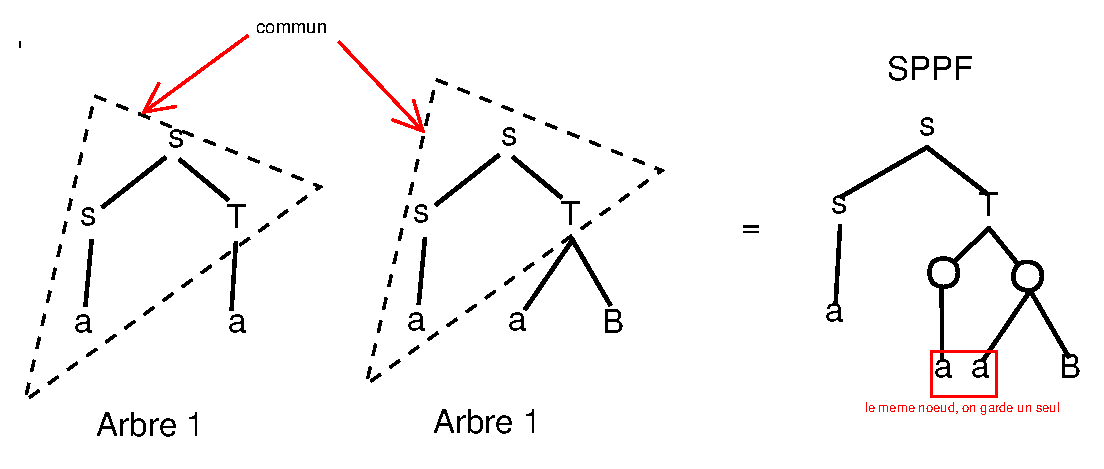
\includegraphics[width=10cm]{Diagramme2.eps}

\section{Earley Alogirithme}
Prenons cette grammaire:
\begin{lstlisting}
S = S + P
| P
P = P * F
| F
F = ( S )
| n
\end{lstlisting}

on veux reconnaitre l'entrée

\begin{tabular}{|l|l|l|l|l|l|l|}
	\hline
	n & + & ( & n & * & n & ) \\ \hline
\end{tabular}

A l'étape 0, le calcule démarre avec l'ensemble E(0) et les règles de l'axiome 'S'


\begin{tabular}{|c|}
	\hline
	\textbf{E(0)}                                                       \\ \hline
	\begin{tabular}[c]{@{}c@{}}S = •S + P (0)\\ S = •P (0)\end{tabular} \\ \hline
\end{tabular}

la prédiction du premier item de E(0) nous donnera les mêmes 2 items de E(0), et donc pas besoin de faire quoi que se sois, donc une la grammaire récursive gauche ne posera pas de problème a notre algorithme.

La prédiction du deuxième item de E(0) générera deux nouveaux items:

\begin{tabular}{|c|}
	\hline
	\textbf{E(0)}                                                                                    \\ \hline
	\begin{tabular}[c]{@{}c@{}}S = •S + P (0)\\ S = •P (0)\\ P = •P * F (0)\\ P = •F (0)\end{tabular} \\ \hline
\end{tabular}

Le prédiction du 3ème item de E(0) ne sert a rien. La prédiction du 4ème item de E(0) générera deux nouveaux items supplémentaire:

\begin{tabular}{|c|}
	\hline
	\textbf{E(0)}                                                                                                                   \\ \hline
	\begin{tabular}[c]{@{}c@{}}S = •S + P (0)\\ S = •P (0)\\ P = •P * F (0)\\ P = •F (0)\\ F = •( S ) (0)\\ F = •n (0)\end{tabular} \\ \hline
\end{tabular}

La Lecture du 5ème item de E(0) échoue puisque le symbole ne correspond pas a l'entrée.

La lecture du 6ème item se fait avec succès, est génère un nouveau item dans l'ensemble suivant E(1)

\begin{tabular}{|c|}
	\hline
	\textbf{E(1)} \\ \hline
	F = n• (0)    \\ \hline
\end{tabular}

On a traité tout les items de E(0), attaquons nous a l'ensemble E(1)

La Complétion du premier item de E(1), nous fait ajouter le 4ème item de E(0) a E(1):

\begin{tabular}{|c|}
	\hline
	\textbf{E(1)}                                                   \\ \hline
	\begin{tabular}[c]{@{}c@{}}F = n• (0)\\ P = F• (0)\end{tabular} \\ \hline
\end{tabular}

la Complétion du deuxième item de E(1), nous fait ajouter le deuxième et troisième item de E(0) dans E(1)

\begin{tabular}{|c|}
	\hline
	\textbf{E(1)}                                                                                 \\ \hline
	\begin{tabular}[c]{@{}c@{}}F = n• (0)\\ P = F• (0)\\ S = P• (0)\\ P = P• * F (0)\end{tabular} \\ \hline
\end{tabular}

...

Au finale notre table Earley ressemblera a :

\begin{tabular}{lllllllll}
	\cline{1-1} \cline{3-3} \cline{5-5} \cline{7-7} \cline{9-9}
	\multicolumn{1}{|c|}{\textbf{E(0)}}                                                                                                                   & \multicolumn{1}{c|}{\textbf{}} & \multicolumn{1}{c|}{\textbf{E(1)}}                                                                                                                       & \multicolumn{1}{c|}{}          & \multicolumn{1}{c|}{\textbf{E(2)}}                                                                                                      & \multicolumn{1}{l|}{} & \multicolumn{1}{c|}{\textbf{E(3)}}                                                                                                                                    & \multicolumn{1}{c|}{\textbf{}} & \multicolumn{1}{c|}{\textbf{E(4)}}                                                                                                                   \\ \cline{1-1} \cline{3-3} \cline{5-5} \cline{7-7} \cline{9-9} 
	\multicolumn{1}{|l|}{\begin{tabular}[c]{@{}l@{}}S = •S + P (0)\\ S = •P (0)\\ P = •P * F (0)\\ P = •F (0)\\ F = •( S ) (0)\\ F = •n (0)\end{tabular}} & \multicolumn{1}{l|}{}          & \multicolumn{1}{l|}{\begin{tabular}[c]{@{}l@{}}F = n• (0)\\ P = F• (0)\\ S = P• (0)\\ P = P• * F (0)\\ S = S• + P (0)\end{tabular}}                      & \multicolumn{1}{l|}{}          & \multicolumn{1}{l|}{\begin{tabular}[c]{@{}l@{}}S = S + •P (0)\\ P = •P * F (2)\\ P = •F (2)\\ F = •( S ) (2)\\ F = •n (2)\end{tabular}} & \multicolumn{1}{l|}{} & \multicolumn{1}{l|}{\begin{tabular}[c]{@{}l@{}}F = ( •S ) (2)\\ S = •S + P (3)\\ S = •P (3)\\ P = •P * F (3)\\ P = •F (3)\\ F = •( S ) (3)\\ F = •n (3)\end{tabular}} & \multicolumn{1}{l|}{}          & \multicolumn{1}{l|}{\begin{tabular}[c]{@{}l@{}}F = n• (3)\\ P = F• (3)\\ S = P• (3)\\ P = P• * F (3)\\ S = S• + P (3)\\ F = ( S• ) (2)\end{tabular}} \\ \cline{1-1} \cline{3-3} \cline{5-5} \cline{7-7} \cline{9-9} 
	&                                &                                                                                                                                                          &                                &                                                                                                                                         &                       &                                                                                                                                                                       &                                &                                                                                                                                                      \\ \cline{1-1} \cline{3-3} \cline{5-5}
	\multicolumn{1}{|c|}{\textbf{E(5)}}                                                                                                                   & \multicolumn{1}{c|}{\textbf{}} & \multicolumn{1}{c|}{\textbf{E(6)}}                                                                                                                       & \multicolumn{1}{c|}{\textbf{}} & \multicolumn{1}{c|}{\textbf{E(7)}}                                                                                                      &                       &                                                                                                                                                                       &                                &                                                                                                                                                      \\ \cline{1-1} \cline{3-3} \cline{5-5}
	\multicolumn{1}{|l|}{\begin{tabular}[c]{@{}l@{}}P = P * •F (3)\\ F = •( S ) (5)\\ F = •n (5)\end{tabular}}                                            & \multicolumn{1}{l|}{}          & \multicolumn{1}{l|}{\begin{tabular}[c]{@{}l@{}}F = n• (5)\\ P = P * F• (3)\\ S = P• (3)\\ P = P• * F (3)\\ F = ( S• ) (2)\\ S = S• + P (3)\end{tabular}} & \multicolumn{1}{l|}{}          & \multicolumn{1}{l|}{{\color[HTML]{333333} \begin{tabular}[c]{@{}l@{}}F = ( S )• (2)\\ P = F• (2)\\ S = S + P• (0)\end{tabular}}}        &                       &                                                                                                                                                                       &                                &                                                                                                                                                      \\ \cline{1-1} \cline{3-3} \cline{5-5}
\end{tabular}

Le mot est reconnu uniquement si on a un item de la forme (S = $\alpha$ • (0)) dans E(7), ce qui est le cas dans notre exemple.

\section{Essayant de construire un l'Analyseur Earley}
Earley lui même a donné un brève description sur comment construire une représentation de tout les dérivations possible a partir de l'algorithme de base qui ne fais que de la reconnaissance. Et il dit aussi que sa ne requière qu'une complexité cubique en temps et en mémoire au pire des cas.

L'idée de Earley est très simple, a chaque fois qu'on fait une complétion, on ajoute un pointeur depuis chaque symbole non terminale a gauche du point du nouveau item, vers les items qui ont engendrés cette item.

Prenons cette grammaire:
\begin{lstlisting}
S = S T 
  | a ;
B = ;
T = a B 
  | a ;
\end{lstlisting}
On applique l'idée d'Earley précédente pour reconnaitre le mot \lstinline|aa|, on aura:

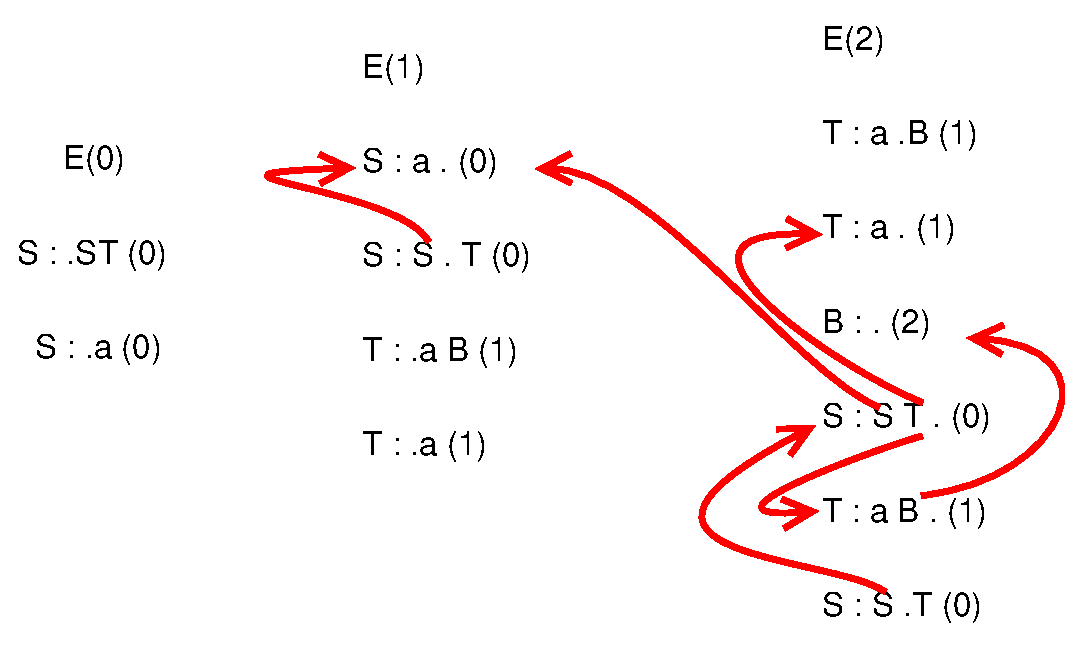
\includegraphics[width=8cm]{Diagramme1.eps}

Ce qui se traduira par la représentation SPPF suivante:

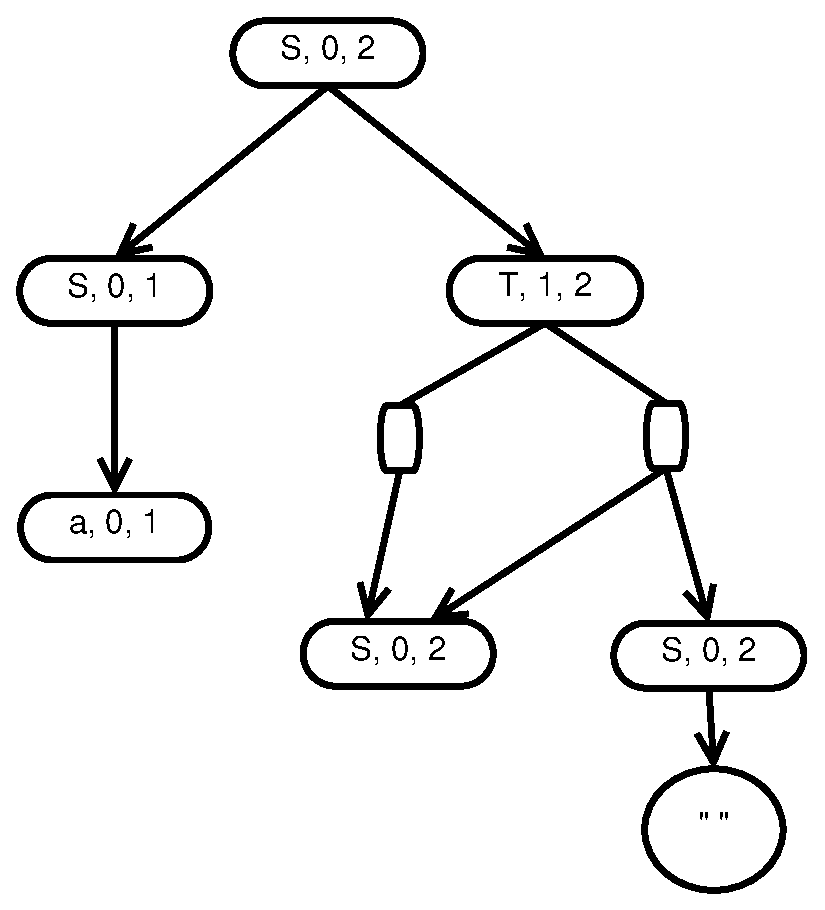
\includegraphics[width=6cm]{Diagramme3.eps}

On vois bien que cette représentation inclue bien tout les dérivations possible du mot \lstinline|aa|, on va pouvoir se dire qu'on a trouver notre algorithme d'analyse syntaxique basé sur Earley, malheureusement, dans certain cas, cette modification de l'algorithme d'Earley pour le transformer en analyseur syntaxique, n'ai pas suffisant. 

Prenons un autre exemple pour démontrer sa:
\begin{lstlisting}
S = SSS 
  | SS
  | b;
\end{lstlisting}

On appliquant la modification d'Earley sur le mot \lstinline|bbb| on aura le SPPF suivant:

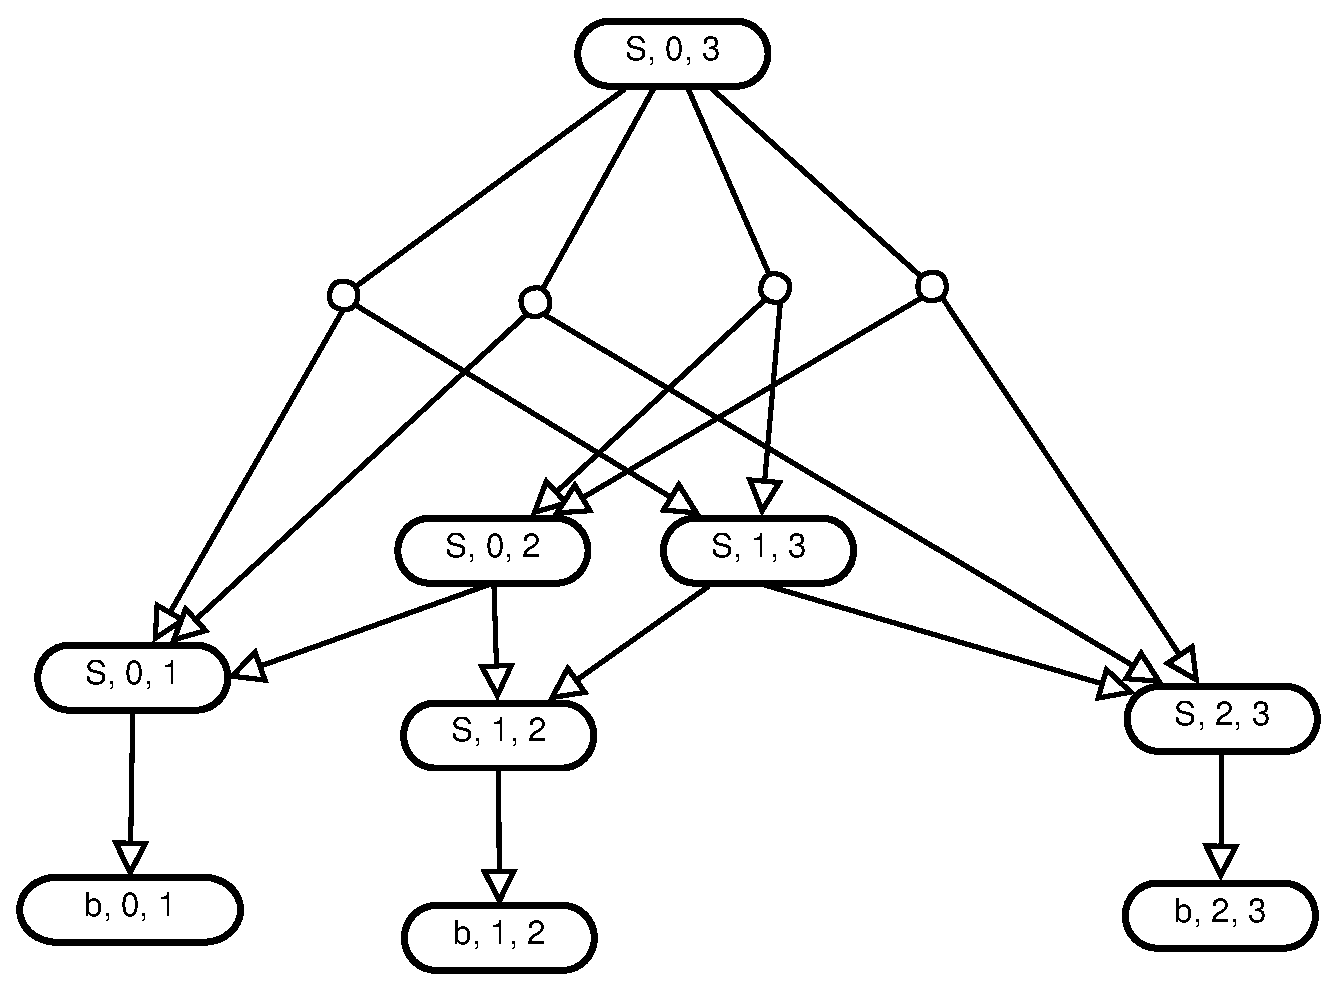
\includegraphics[width=6cm]{Diagramme4.eps}

Cette représentation SPPF contient des dérivations superflus qui sert a reconnaitre les mot \lstinline|bb| et \lstinline|bbbb|, alors que nous voulions juste connaitre les dérivations du mot \lstinline|bbb|. Dans la page 74\cite{Tomita}, Tomita nous explique qu'ajouter plusieurs pointeurs a la même instance du symbole non terminale est une mauvaise idée et résulte sur des dérivation superflus d'autre mot.

Il existe une solution très simple a ce problème. il suffit de dupliquer la règle qui cause se problème. Dans l'exemple précédent, on aura deux règles "S = SS • (0)" identique dans E(3) mais avec des pointeurs différents, ce qui engendrera cette représentation SPPF:

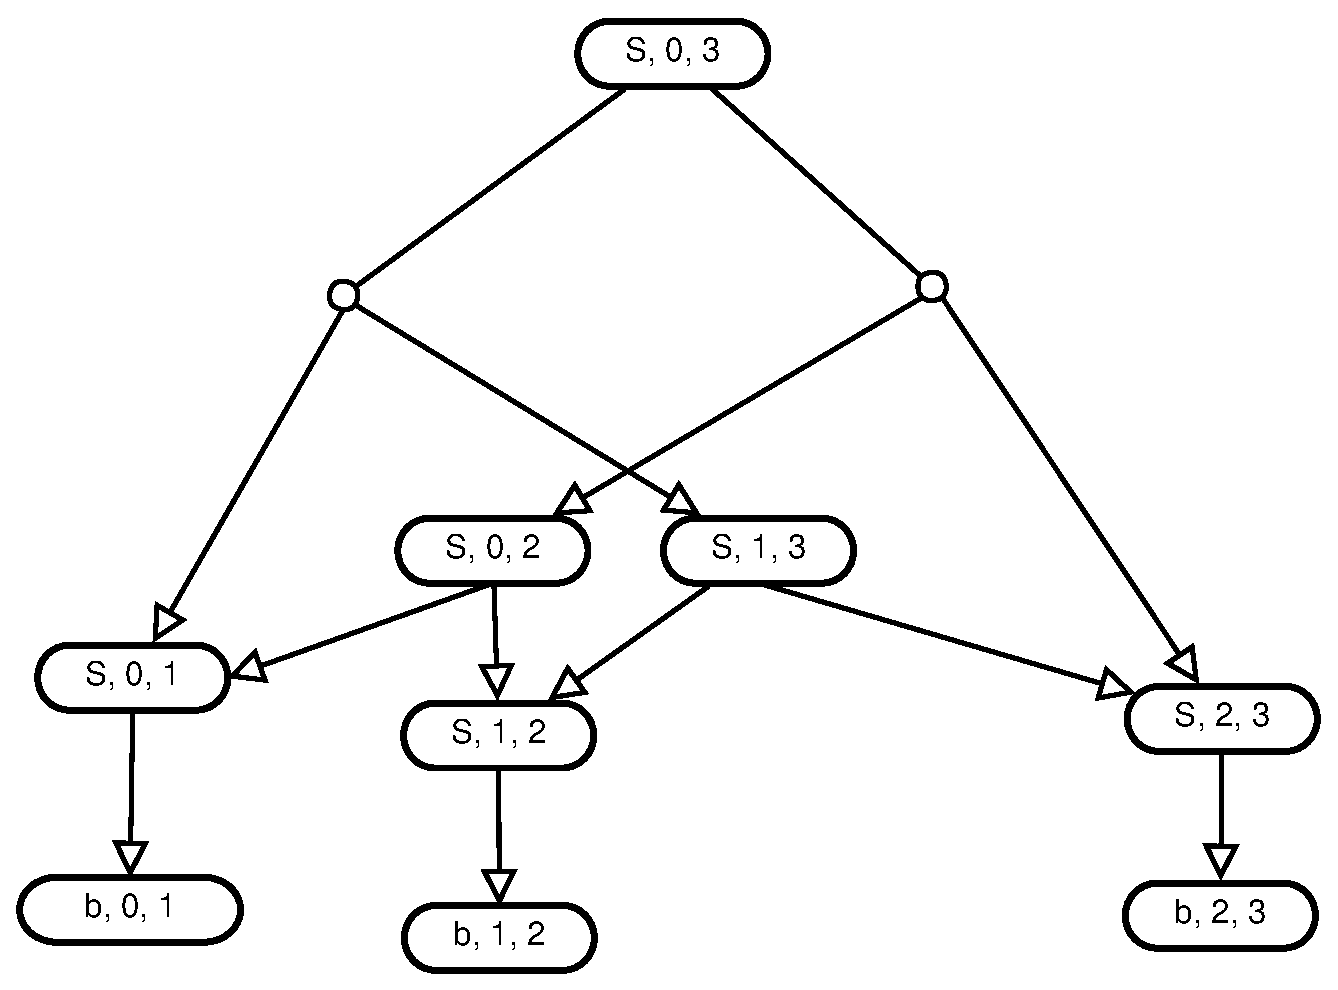
\includegraphics[width=6cm]{Diagramme5.eps}

cette fois si c'est la bonne, la duplication de la règle problématique a permis d'exclure les dérivations superflu.

On viens de trouver un algorithme d'analyse syntaxique basé sur Earley, mais quand est-il de la complexité ? Ben, comme démontrer par Johnson\cite{Johnson} pour un problème similaire et comme confirmé par Scott\cite{Scott}, la complexité polynomiale est infinie. On peut se dire qu'on a gardé l'algorithme de base d'Earley et donc la complexité aurais du être $O(n^3)$, mais la duplication des règles engendrent un problème, en effet, la taille de la table d'Earley ne peut être borné par $O(n^p)$ pour n'importe quelle entier p. Et puisque la complexité en taille et en temps sont liées, on aura une complexité polynomiale infinie.

\chapter{L'algorithme}
Dans cette section, nous allons nous baser sur l'algorithme d'Earley de base et les travaux de Scott\cite{Scott} ainsi que la conclusion de la précédente section, pour donner un algorithme qui sera de complexité $O(n^3)$ en temps et en mémoire. Il sera ensuite utilisé par notre programme que nous décrivons dans les sections suivantes.

Scott c'est rendu compte que il suffit d'ajouter des pointeurs entre items pour pouvoir crée un analyseur syntaxique d'Earley. les pointeur seront nommé pour pouvoir construire la structure SPPF en une seule itération. 

Scott définit deux types de pointeur, un pointeur de réduction, et un pointeur de décalage qui font allusion au opération shift/reduce dans les autres algorithmes d'analyse syntaxique.

L'idée est de d'abord crée la table Earley décoré avec ces fameux pointeurs , ensuite on fait une seule itération sur cette table pour déduire la représentation SPPF (la foret) de toutes les dérivations possibles.

\section{Création de la table d'Earley}
Les opérations de base du reconnaisseur Earley, qui sont: prédiction, lecture et complétion vont être remplacer avec d'autre opérations.

\begin{itemize}
	\item Mettre dans $E_0$ tout item de la forme (S ::= •$\alpha$, 0) qui appartient au règles de la grammaire
	\item Pour chaque $i > 0$, faire l'étape d'initialisation 
	\item Avant d'initialiser $E_{i+1}$, il faut faire l'étape de prédiction et l'étape de complétion a $E_{i}$.
\end{itemize}

Donc on aura les trois étapes suivantes: initialisation, prédiction et complétion. La prédiction sera exactement la même que dans l'algorithme de base d'Earley, par contre la complétion sera modifier pour permettre l'ajout de pointeur.

\section{L'Initialisation}
L'initialisation sera faite a tout les ensembles sauf $E_0$, voici l'algorithme qui décrit cette opération:

Soit le mot a reconnaitre $a_0 a_1 ... a_n$. 

On ajoute $p = (A ::= \alpha a_i • \beta, j)$ pour chaque $q = (A ::= \alpha • a_i \beta, j)$ appartenant a $E_{i-1}$

Si $\alpha \neq \epsilon$ alors crée un pointeur de décalage nommé $i-1$ de $q$ vers $p$.

Donc l'initialisation ressemble a l'algorithme de lecture avec on plus, des pointeur pour trouver l'origine de cette lecture.

\section{La Prédiction}
La prédiction reste exactement la même que dans l'algorithme de base:

Pour chaque item $(B :== \gamma • D \delta, k)$ appartenant a $E_i$ et pour chaque règle de grammaire de la forme $D :== \rho$, on ajoute a $E_i$ l'item $(D :== • \rho, i)$

\section{La Complétion}
La complétion est la même que celle de l'algorithme de base, mais il faut ajouter deux types d'informations pour chaque complétion, a savoir, d'ou on a fait la complétion et grâce a qui on la fait. L'algorithme deviendra comme ceci:

Pour chaque item $t = (B :== \tau, k)$ appartenant a $E_i$ et pour chaque item correspondant $q = (D ::= \alpha • B \mu, h)$ appartenant a $E_k$, si $p = (D ::= \alpha B • \mu, h)$ n'ai pas présent dans $E_i$ alors ajouter p a $E_i$.

On ajoute un pointeur de réduction nommé $k$ de $p$ a $t$

Si $\tau \neq \epsilon$, On ajoute un pointeur de décalage nommé aussi $k$ de $p$ a $q$.

\section{L'Algorithme de construction de la représentation SPPF}
Scott\cite{Scott} avait proposer un algorithme récursive pour passé de la table d'Earley décoré avec des pointeurs a la représentation SPPF, mais après un test, il s'avère qu'il comportait une erreur, qu'on a corrigé
Voici la version corrigé :
\begin{lstlisting}[frame=single]
Buildtree(u, p) 
{
	suppose that ¤$p \in E_i$¤ and that p is of the form ¤$(A ::= \alpha • \beta, j)$¤
	
	mark ¤$p$¤ as processed
	
	if ¤$p =(A ::= •,j)$¤ {
		if ¤$u$¤ does not have a child node ¤$\epsilon$¤ then add a child node ¤$\epsilon$¤ to ¤$u$¤ }
		
	if ¤$p =(A ::= \alpha • \beta, j)$¤ (where ¤$a$¤ is a terminal) {
		if there is no SPPF node ¤$v$¤ labelled ¤$(a, i − 1,i)$¤ create one
		if ¤$u$¤ does not have a family ¤$(v)$¤ then add the family ¤$(v)$¤ to ¤$u$¤ }
		
	if ¤$p =(A ::= C • \beta, j)$¤ (where ¤$C$¤ is a non-terminal) {
		if there is no SPPF node ¤$v$¤ labelled ¤$(C, j, i)$¤ create one
		if ¤$u$¤ does not have a family ¤$(v)$¤ then add the family ¤$(v)$¤ to ¤$u$¤ 
		for each reduction pointer from ¤$p$¤ labelled ¤$j$¤ {
			suppose that the pointer points to ¤$q$¤
			if ¤$q$¤ is not marked as processed ¤$Buildtree(v,q)$¤ } }
			
			
	if ¤$p =(A ::= \alpha' a • \beta, j)$¤ (where a is a terminal, ¤$\alpha' \neq \epsilon$¤) {
		if there is no SPPF node ¤$v$¤ labelled ¤$(a, i − 1,i)$¤ create one
		if there is no SPPF node ¤$w$¤ labelled ¤$(A ::= \alpha' • a \beta, j, i − 1)$¤ create one
		for each target ¤$p'$¤ of a predecessor pointer labelled ¤$i − 1$¤ from ¤$p$¤ {
			if ¤$p'$¤ is not marked as processed ¤$Buildtree(w,p')$¤ }
		if ¤$u$¤ does not have a family ¤$(w, v)$¤ add the family ¤$(w, v)$¤ to ¤$u$¤ }
			
	if ¤$p =(A ::= \alpha' C • \beta, j)$¤ (where ¤$C$¤ is a non-terminal, ¤$\alpha' \neq \epsilon$¤) {
		for each reduction pointer from ¤$p$¤ {
			suppose that the pointer is labelled ¤$l$¤ and points to ¤$q$¤
			if there is no SPPF node ¤$v$¤ labelled ¤$(C, l, i)$¤ create one
			if ¤$q$¤ is not marked as processed ¤$Buildtree(v,q)$¤
			if there is no SPPF node ¤$w$¤ labelled ¤$(A ::= \alpha' • C \beta, j, l)$¤ create one 
			for each target ¤$p'$¤ of a predecessor pointer labelled ¤$l$¤ from ¤$p$¤ {
				if ¤$p'$¤ is not marked as processed ¤$Buildtree(w,p')$¤ }
			if ¤$u$¤ does not have a family ¤$(w, v)$¤ add the family ¤$(w, v)$¤ to ¤$u$¤ }}
}
		
		
\end{lstlisting}

Et Pour construire la représentation entière depuis la racine, on exécute la fonction suivante: 

\begin{lstlisting}[frame=single]		
PARSER { 
	create an SPPF node ¤$u0$¤ labelled ¤$(S, 0, n)$¤
	for each decorated item ¤$p =(S ::= \alpha •, 0) \in E_n$¤ ¤$Buildtree(u0, p)$¤ 
}
\end{lstlisting}

\section{Problème de la règle nulle}
l'algorithme précédent est parfait, néanmoins, on remarque qu'il y a un problème pour construire la table Earley (la version décoré avec des pointeurs) quand il y a des symboles annulable dans la grammaire.

Prenons un exemple de grammaire pour illustrer le problème:
\begin{lstlisting}		
A :== ¤$\epsilon$¤
A :== B
B :== A
\end{lstlisting}

Si nous construisons notre table Earley pour reconnaitre le mot vide, on aura le résultat suivant:
\begin{lstlisting}
   E(0)	
A :== • (0)
A :== •B (0)
B :== •A (0)
\end{lstlisting}
et nous aurons le graphe SPPF suivant:

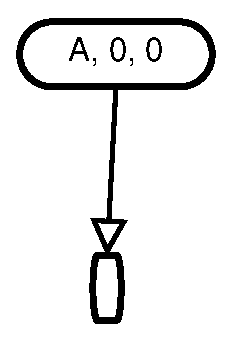
\includegraphics[width=1.5cm]{Diagramme6.eps}

il manque deux item dans notre ensemble $E_0$, a savoir \lstinline|A :== B • (0)| et \lstinline|B :== A • (0)|.

Le problème vient d'un mauvais timing pour faire l'opération de complétion. En effet, au moment de compléter \lstinline|A :== • (0)|, l'item \lstinline|B :== •A (0)| n'ai pas encore présent dans $E_0$.

Pour résoudre ce problème, il ya la méthode simple qui consiste a faire plusieurs itérations de complétion et de prédiction sur chaque ensemble $E_i$ jusqu'à aucun item n'ai ajouté. Plusieurs itération signifie complexité dans le pire cas va s'envoler, et donc on utilisera pas cette méthode.

La solution a ce problème est donné par Aycock et Horspool\cite{Aycock}. Ils ont remarqué qu'il pouvait faire avancer certain items sans attendre de faire une complétion. Plus précisément, au moment de la prédiction de $q = (B :== \alpha • C \tau, k) \in E_i$, si $C$ est annulable, alors on ajoute aussi $q = (B :== \alpha C • \tau, k)$ a $E_i$. On appellera cette opération, la prédiction magique.

Cette solution n'ai pas complète encore, puisque il faut aussi mettre les différents pointeurs de réduction a ces nouveaux items issu de la prédiction magique. L'idée est de marqué l'item suite a une redirection magique. Ensuite a la fin du des opérations de prédictions et de complétions sur $E_i$, on parcours tout les items marqué (suite une prédiction magique) et on complète les pointeur de réductions qui manque.

\section{Détecter qu'un symbole est annulable}
Le réel problème maintenant est de trouver (ou crée) un algorithme pour détecter les symboles annulables et que sa complexité, doit être inférieur a $O(n_3)$, qui est la complexité de l'analyseur syntaxique Earley.

Il s'avère que la solution est simple, On va lire chaque règle de la grammaire, et maintenir une liste de symbole annulable qu'on a trouvé. Si une règle est annulable ou bien contient uniquement des symbole annulable (dans sa parti droite), alors on ajoute le symbole du gauche de cette règle a cette liste, et on recommence le processus, jusqu'à aucun symbole n'ai rajouté.

Cette algorithme est largement suffisant pour notre analyseur Earley et a une complexité quadratique $O(n_2)$ par rapport a la taille de la grammaire.

Il s'avère qu'il existe un meilleur algorithme pour ce problème, avec une complexité linaire $O(n)$. Il a été documenté dans les pages 293-295 du livre sur Marpa\cite{Marpa}. Mais on va pas l'utiliser dans notre programme puisque cette algorithme est assez complexe a implémenter et va grandement diminuer la lisibilité du code.

\chapter{Le programme}
Dans cette section, je vais mettre tout ce qui a un rapport avec le programme que j'ai développer. A savoir, comment l'utiliser, le diagramme de classe et les différente dépendance de notre programme.
\section{Utiliser le programme}
Le projet se trouve sur Github\footnote{https://github.com/rezid/earley}. C'est le dossier "code" qui contient le code source du programme.

Pour compiler le programme, il faut d'abord installer les dépendances :
\begin{lstlisting}
$ sudo apt-get update
$ sudo apt-get install graphviz
\end{lstlisting}

Ensuite :

\begin{lstlisting}
$ git clone ¤https://github.com/rezid/earley.git¤
$ cd earley
$ cd code
$ make
\end{lstlisting}

Cela compilera le programme et créera l'exécutable \lstinline|bin/app.out|.

Pour exécuter le programme, on a besoin de deux fichiers. Le premier qui contient la définition de la grammaire, il faut faire attention a bien séparer les symboles par des espaces:
\begin{lstlisting}
%token ¤the a this he she book boys girl with in takes take¤;

S : NP VP | Aux NP VP | VP;
NP : PRON | Det Nom;
Nom : N | Nom N | Nom PP;
PP : PRP NP;
VP : V  | V NP | VP PP;
Det : ¤the¤ | ¤a¤ | ¤this¤;
PRON : ¤he¤ | ¤she¤;
N : ¤book¤ | ¤boys¤ | ¤girl¤;
PRP : ¤with¤ | ¤in¤;
V : ¤takes¤ | ¤take¤;
\end{lstlisting}
et le deuxième fichier contient le mot a analyser séparé par des espace:
\begin{lstlisting}
¤take this book¤
\end{lstlisting}

il suffit d'exécuter la commande suivante:
\begin{lstlisting}
$ .bin/app.out grammar.txt string.txt
\end{lstlisting}

Deux cas peuvent se produire. Sois le mot n'ai pas reconnu est dans ce cas le message suivant s'affiche sur la console:
\begin{lstlisting}
PARSE FAIL : word does not belong to the grammar 
\end{lstlisting}

Sois le mot est reconnu par la grammaire et dans ce cas la, le PDF contenant le graphe SPPF du mot s'affiche.

Voici un diagramme de classe comportent uniquement les noms des classes utilisés et leurs relations.

\section{Diagramme De Classe}
Voici un diagramme de classe comportent uniquement les noms des classes utilisés et leurs relations, le lecteur doit connaitre la différence entre une agrégation et une composition pour lire correctement le diagramme.

\begin{tikzpicture}
\begin{class}[text  width=2cm]{Grammar}{3,0}
\end{class}

\begin{class}[text  width=2cm]{Rule}{8,0}
\end{class}

\begin{class}[text  width=2cm]{EarleyTable}{0,-3}
\end{class}

\begin{class}[text  width=2cm]{EarleySet}{8,-3}
\end{class}

\begin{class}[text  width=2cm]{EarleyItem}{15,-3}
\end{class}

\begin{class}[text  width=3cm]{EarleyItemPtr}{3,-6}
\end{class}

\begin{class}[text  width=3cm]{EarleyItemPtrList}{9,-6}
\end{class}

\begin{class}[text  width=2cm]{ItemCategory}{14,-6}
\end{class}

\begin{class}[text  width=2cm]{Tree}{0,-9}
\end{class}

\begin{class}[text  width=2cm]{Node}{7,-9}
\end{class}

\composition{Grammar}{ rule\_list }{1..*}{Rule}
\aggregation{EarleyTable}{ grammar }{1}{Grammar}
\composition{EarleyTable}{ table }{1..*}{EarleySet}
\composition{EarleySet}{ set }{1..*}{EarleyItem}
\aggregation{EarleyItem}{ rule\_ptr }{1}{Rule}
\composition{EarleyItem}{ reduction\_ptr\_list predecessor\_ptr\_list }{2}{EarleyItemPtrList}
\composition{EarleyItemPtrList}{ list }{1..*}{EarleyItemPtr}
\aggregation{EarleyItemPtr}{ item\_ptr }{1}{EarleyItem}
\aggregation{Tree}{ table }{1}{EarleyTable}
\composition{Tree}{ node\_list epsilon }{1..*}{Node}
\unidirectionalAssociation{EarleyItem}{}{1}{ItemCategory}
\end{tikzpicture}

Pour pas encombrer le diagramme voici la suite:

\begin{tikzpicture}
\begin{class}[text  width=2cm]{EarleyTable}{0,0}
\end{class}

\begin{class}[text  width=2cm]{EarleySet}{7,0}
\end{class}


\begin{class}[text  width=2cm]{Node1}{0,-2}
\end{class}

\begin{class}[text  width=2cm]{Node2}{7,-2}
\end{class}

\aggregation{EarleySet}{ earley\_table }{1}{EarleyTable}
\aggregation{Node1}{ families }{1}{Node2}
\end{tikzpicture}

remarque que Node1 et Node2 référent a la même classe: Node

\section{La Classe Grammar}
\begin{tikzpicture}
\begin{class}[text  width=9cm]{Grammar}{0,0}

\attribute {start\_symbole : string }
\attribute {terminal\_symbole\_list : list\_of\_string }
\attribute {rule\_list : list\_of\_rule }
\attribute {nullable\_symbole\_list : list\_of\_string }

\operation {Grammar ( )}
\operation {set\_start\_symbole (string)}
\operation {set\_terminal\_symbole\_list (list\_of\_string)}
\operation {add\_rule\_if\_not\_present (rule)}
\operation {add\_terminal\_symbole\_if\_not\_present (string)}
\operation {add\_nullable\_symbole\_if\_not\_present (string)}
\operation {get\_rule\_list ( )}
\operation {get\_start\_symbole ( )}
\operation {print\_terminal\_symbole\_list ( )}
\operation {print\_rule\_list ( )}
\operation {print\_nullable\_symbole\_list ( )}
\operation {is\_terminal\_symbole (string)}
\operation {is\_not\_terminal\_symbole (string)}
\operation {is\_nullable\_symbole (string)}
\operation {compute\_nullable\_symbole\_list( )}
\operation {create\_earley\_table\_from\_input(reference of string\_list)}
\end{class}
\end{tikzpicture}

Cette classe représente une grammaire, elle comporte toute les constituantes de cette derniers, a savoir: 
\begin{itemize}
	\item Les symbole terminaux
	\item Les règles
	\item Le symbole de départ
\end{itemize}
On a ajouté dans cette classe la liste des symboles annulables.


\section{La Classe Rule}
\begin{tikzpicture}
\begin{class}[text  width=6cm]{Rule}{0,0}

\attribute {main\_symbole : string }
\attribute {body : list\_of\_string }
\attribute {main\_symbole\_is\_set : boolean }

\operation {Rule ( )}
\operation {Rule (string, list\_of\_string)}
\operation {print\_rule (string)}
\operation {print\_Earley\_rule (integer, integer)}
\operation {get\_main\_symbole ( )}
\operation {get\_symbole (integer)}
\operation {set\_main\_symbole (string)}
\operation {set\_body (list\_of\_string)}
\operation {get\_body ( )}
\operation {push\_back\_symbole\_to\_body (string)}
\operation {clear\_rule ( )}
\operation {clear\_body ( )}
\operation {operator== (reference to rule)}
\operation {size ( )}
\end{class}
\end{tikzpicture}

Cette classe représente une règle de production, elle comporte toute les constituantes de cette derniers, a savoir: 
\begin{itemize}
	\item Le symbole de départ (la partie gauche de la règle).
	\item Le body de la règle (la partie droite de la règle).
\end{itemize}

\section{La Classe EarleyTable}
\begin{tikzpicture}
\begin{class}[text  width=8cm]{EarleyTable}{0,0}

\attribute {table : list\_of\_EarleySet }
\attribute {input\_symbole\_list : list\_of\_string }
\attribute {grammar : reference to Grammar }

\operation {EarleyTable (Grammar, reference to list\_of\_string)}
\operation {add\_item\_to\_set\_if\_not\_present (int, EarleyItem)}
\operation {size ( )}
\operation {get\_input\_symbol (integer)}
\operation {get\_grammar ( )}
\operation {get\_set (integer)}
\operation {compute\_earley\_table ()}
\operation {front ()}
\operation {back ( )}
\operation {print\_table ()}
\operation {generate\_sppf\_structure ( )}
\operation {get\_category (reference to EarleyItem)}
\end{class}
\end{tikzpicture}

Cette classe représente la table d'Earley, elle est constitué de plusieurs ensemble d'Earley (EarleySet), on trouve aussi dans cette classe le mot a reconnaitre, puisque chaque table d'Earley correspond a un mot donné. On garde aussi une référence vert la grammaire utilisé pour calculer la table.

\section{La Classe EarleySet}
\begin{tikzpicture}
\begin{class}[text  width=9cm]{EarleySet}{0,0}

\attribute {set : list\_of\_EarleyItem }
\attribute {index : integer }
\attribute {earley\_table : reference to EarleyTable }
\attribute {precedent\_set : reference to EarleySet }

\operation {EarleySet (reference to EarleySet, reference to EarleyTable)}
\operation {magical\_prediction (reference to EarleyItem)}
\operation {prediction (EarleyItem)}
\operation {completion (reference to EarleyItem)}
\operation {set\_precedent\_set (reference to EarleySet)}
\operation {get\_set ( )}
\operation {add\_item\_if\_not\_present (reference to EarleyItem)}
\operation {front ()}
\operation {size ( )}
\operation {print\_set ()}
\operation {initialize ( )}
\operation {complete ( )}
\operation {resolve\_magical\_prediction\_reduction\_ptr ( )}
\operation {get\_index ( )}
\end{class}
\end{tikzpicture}

Cette classe représente une ensemble d'Earley, elle est constitué de plusieurs item (EarleyItem), chaque ensemble garde en mémoire une référence vers le précédent ensemble forment ainsi une liste chainé. Chaque ensemble possède aussi un index (Pour $E_0$ l'index c'est $0$). On garde aussi une référence vers la table d'Earley ou appartient l'ensemble, histoire de pouvoir remonter vers la table si besoin.

\section{La Classe EarleyItem}
\begin{tikzpicture}
\begin{class}[text  width=9cm]{EarleyItem}{0,0}

\attribute {rule\_ptr : reference to Rule }
\attribute {position : integer }
\attribute {item\_start : integer }
\attribute {reduction\_ptr\_list : EarleyItemPtrList }
\attribute {predecessor\_ptr\_list : EarleyItemPtrList }
\attribute {symbole\_before\_position\_is\_null : boolean }
\attribute {from\_magical\_reduction : boolean }
\attribute {processed : boolean }

\operation {EarleyItem (reference to Rule, integer, integer, boolean)}
\operation {next\_symbole ( )}
\operation {precedent\_symbole ( )}
\operation {print\_item ( )}
\operation {print\_item\_without\_pointer ( )}
\operation {operator== (reference to EarleyItem)}
\operation {next\_item (boolean)}
\operation {get\_item\_start ()}
\operation {get\_position ()}
\operation {get\_rule ()}
\operation {add\_reduction\_ptr (EarleyItemPtr)}
\operation {add\_predecessor\_ptr (EarleyItemPtr)}
\operation {get\_reduction\_ptr\_list( )}
\operation {get\_predecessor\_ptr\_list( )}
\operation {is\_symbole\_before\_position\_is\_null ( )}
\operation {is\_symbole\_before\_position\_is\_not\_null ()}
\operation {is\_complete ( )}
\operation {is\_from\_magical\_reduction ()}
\operation {set\_from\_magical\_reduction (boolean)}
\operation {set\_processed (boolean)}
\operation {is\_processed ( )}
\operation {is\_not\_processed ( )}
\operation {mark\_as\_processed ( )}
\operation {is\_symbole\_before\_two\_position\_is\_null ( )}
\operation {get\_alpha\_prim ( )}
\operation {get\_beta ( )}
\end{class}
\end{tikzpicture}

Cette classe représente un item, elle comporte toute les constituantes de cette derniers, a savoir: 
\begin{itemize}
	\item La règle de production utilisé 
	\item La position du point
	\item le numéro entre parenthèse
	\item les pointeurs de réduction
	\item les pointeur de décalage
\end{itemize}

\chapter{ANNEXE A: Quelque images produite par le programme}

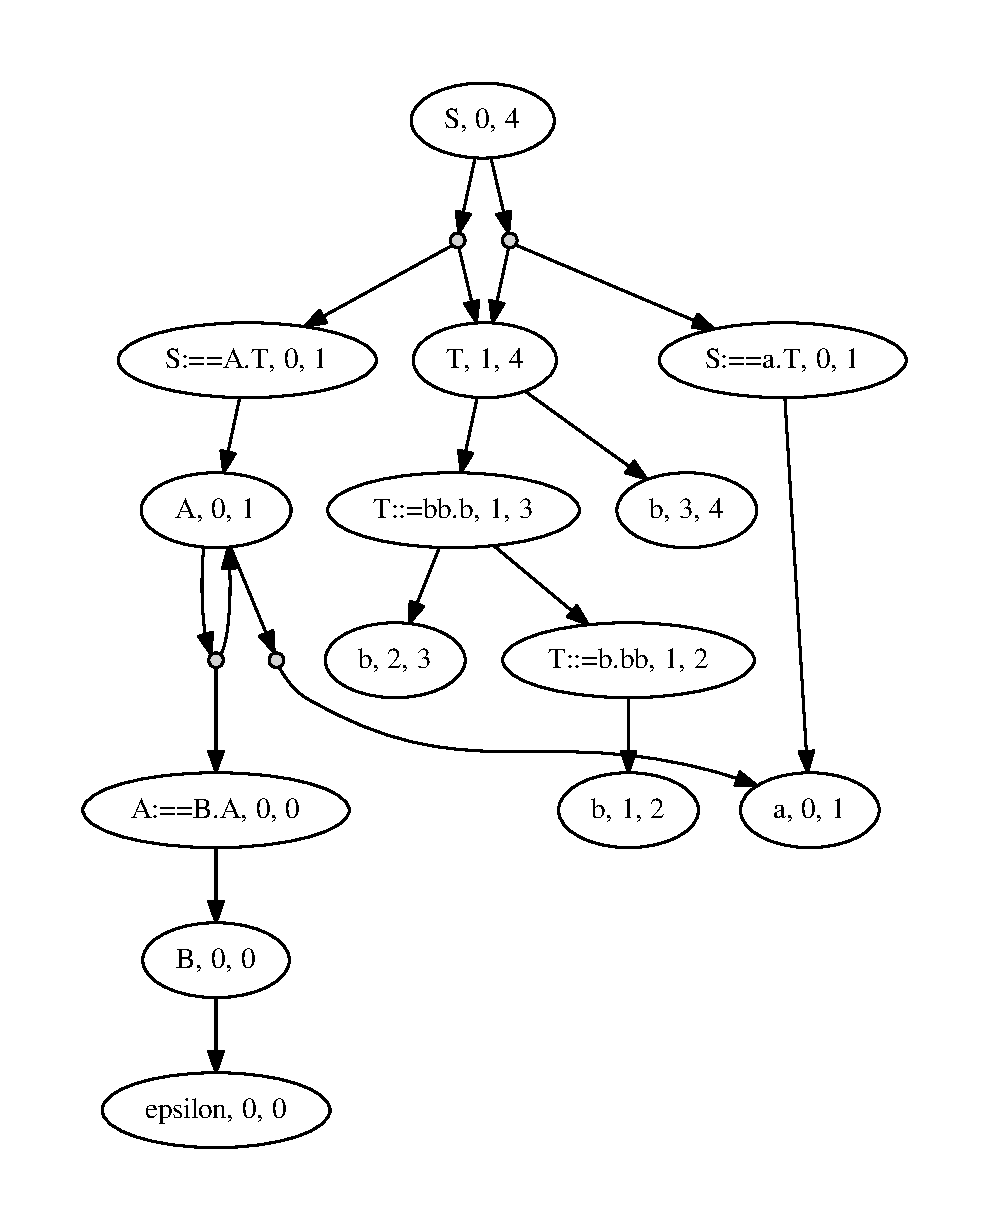
\includegraphics[width=6cm]{ast1.pdf}
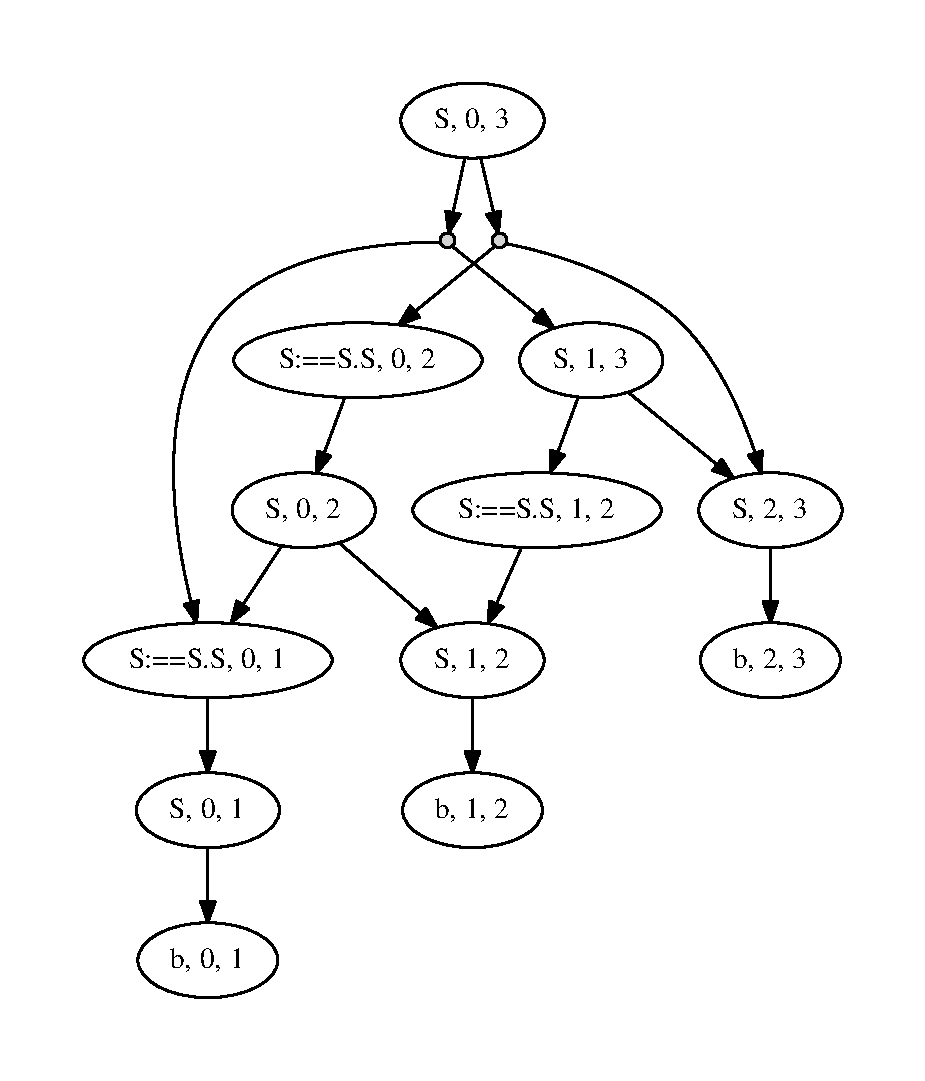
\includegraphics[width=6cm]{ast2.pdf}
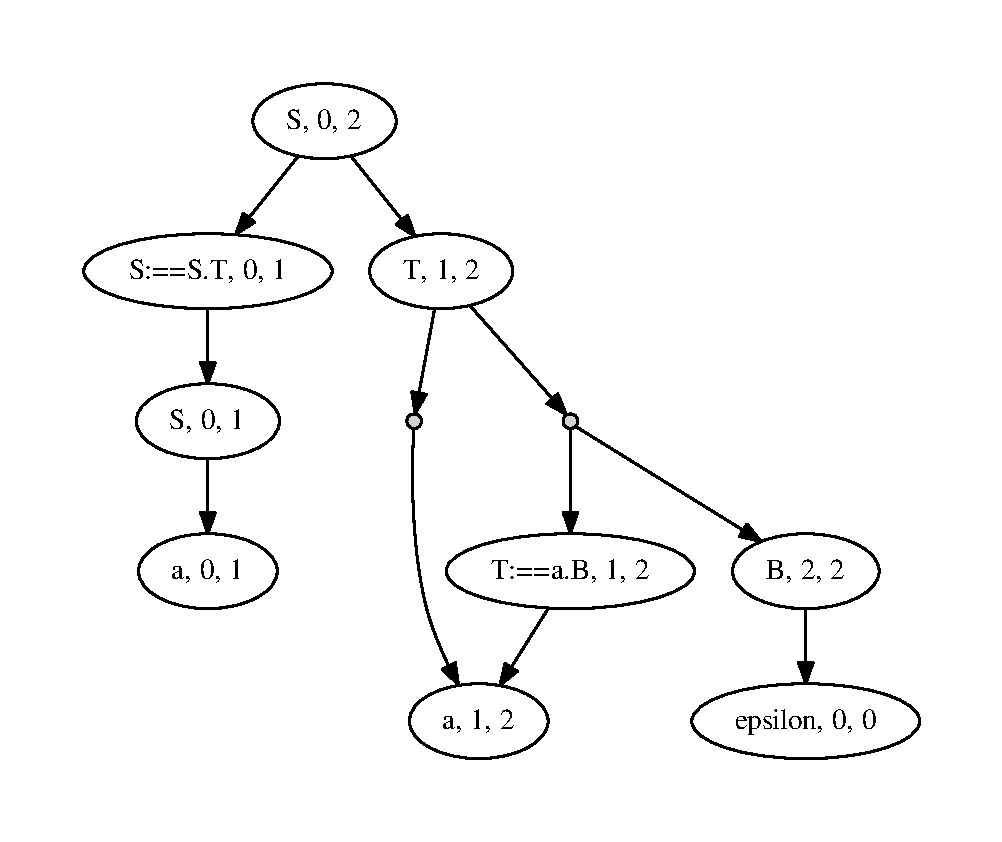
\includegraphics[width=6cm]{ast3.pdf}
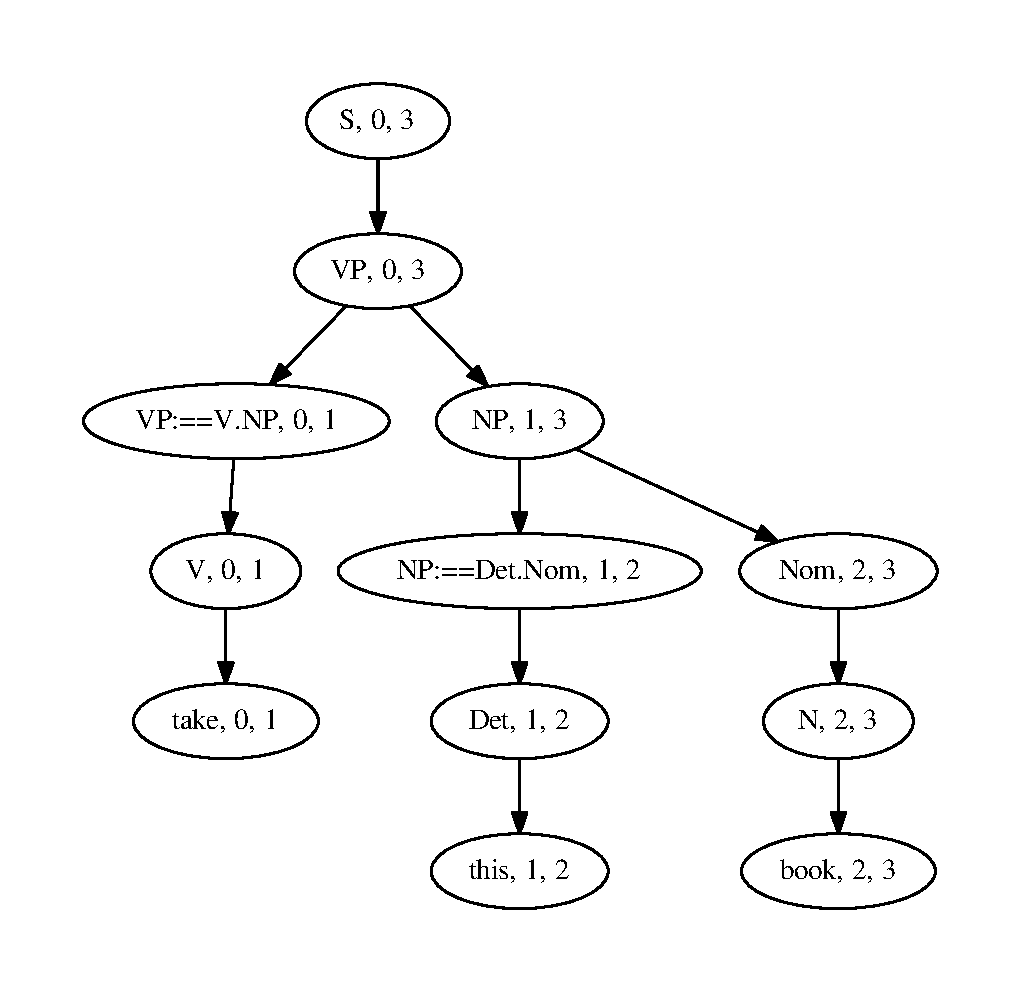
\includegraphics[width=8cm]{ast4.pdf}
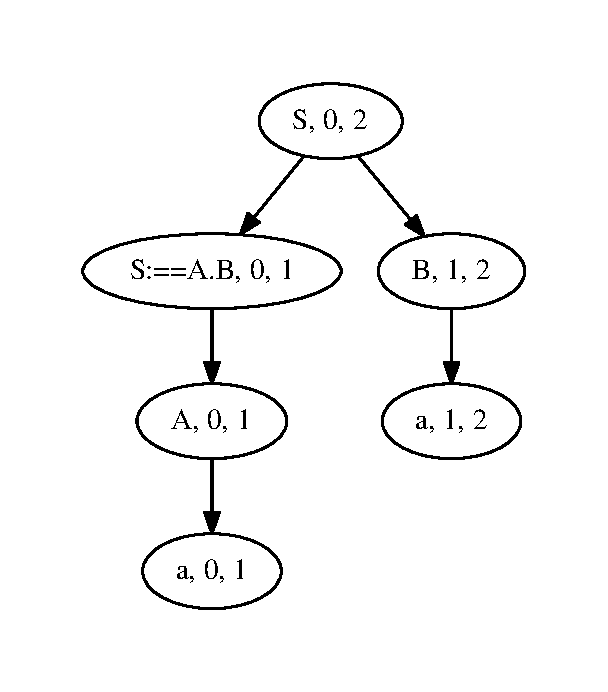
\includegraphics[width=5cm]{ast5.pdf}

\bibliographystyle {plain}
\bibliography{mabiblio}  
\end{document}